\chapter{Installation du Twiz O' Meter sur votre véhicule}

L'installation du ToM+ sur votre Twizy est très simple et ne nécessite aucune connaissance particulière car, comme j'ai l'habitude de le dire, c'est un appareil « plug and drive » (prêt à l'emploi) ! Suivez donc ces quelques étapes pour l'installer correctement et rapidement, ou tentez d'essayer par vous-même un autre emplacement.

\section{Positionnement de l'écran LCD}

Lors de la commande de l'appareil, vous pouvez choisir de recevoir le support 3D avec l'écran à clipser.
Vous pouvez ainsi choisir d'installer l'écran de deux manières différentes : en utilisant le mode à clipser ou en utilisant le mode support 3D. Le mode à clipser est le plus courant et vous permet de fixer l'écran au tableau de bord de la voiture, tandis que le mode support 3D vous permet de placer l'écran sur une surface plane à l'intérieur du véhicule (je suggère généralement la boîte à gants droite ou gauche).

\subsection{Mode à clipser}

Si vous choisissez ce mode, c'est très simple. Il vous suffit de clipser l'écran sur le tableau de bord, dans une position confortable à regarder pendant la conduite. Placez la partie supérieure de l'écran sur le tableau de bord, puis poussez la partie inférieure jusqu'à ce qu'elle s'enclenche avec un déclic.

\begin{figure}[H]
    \centering
    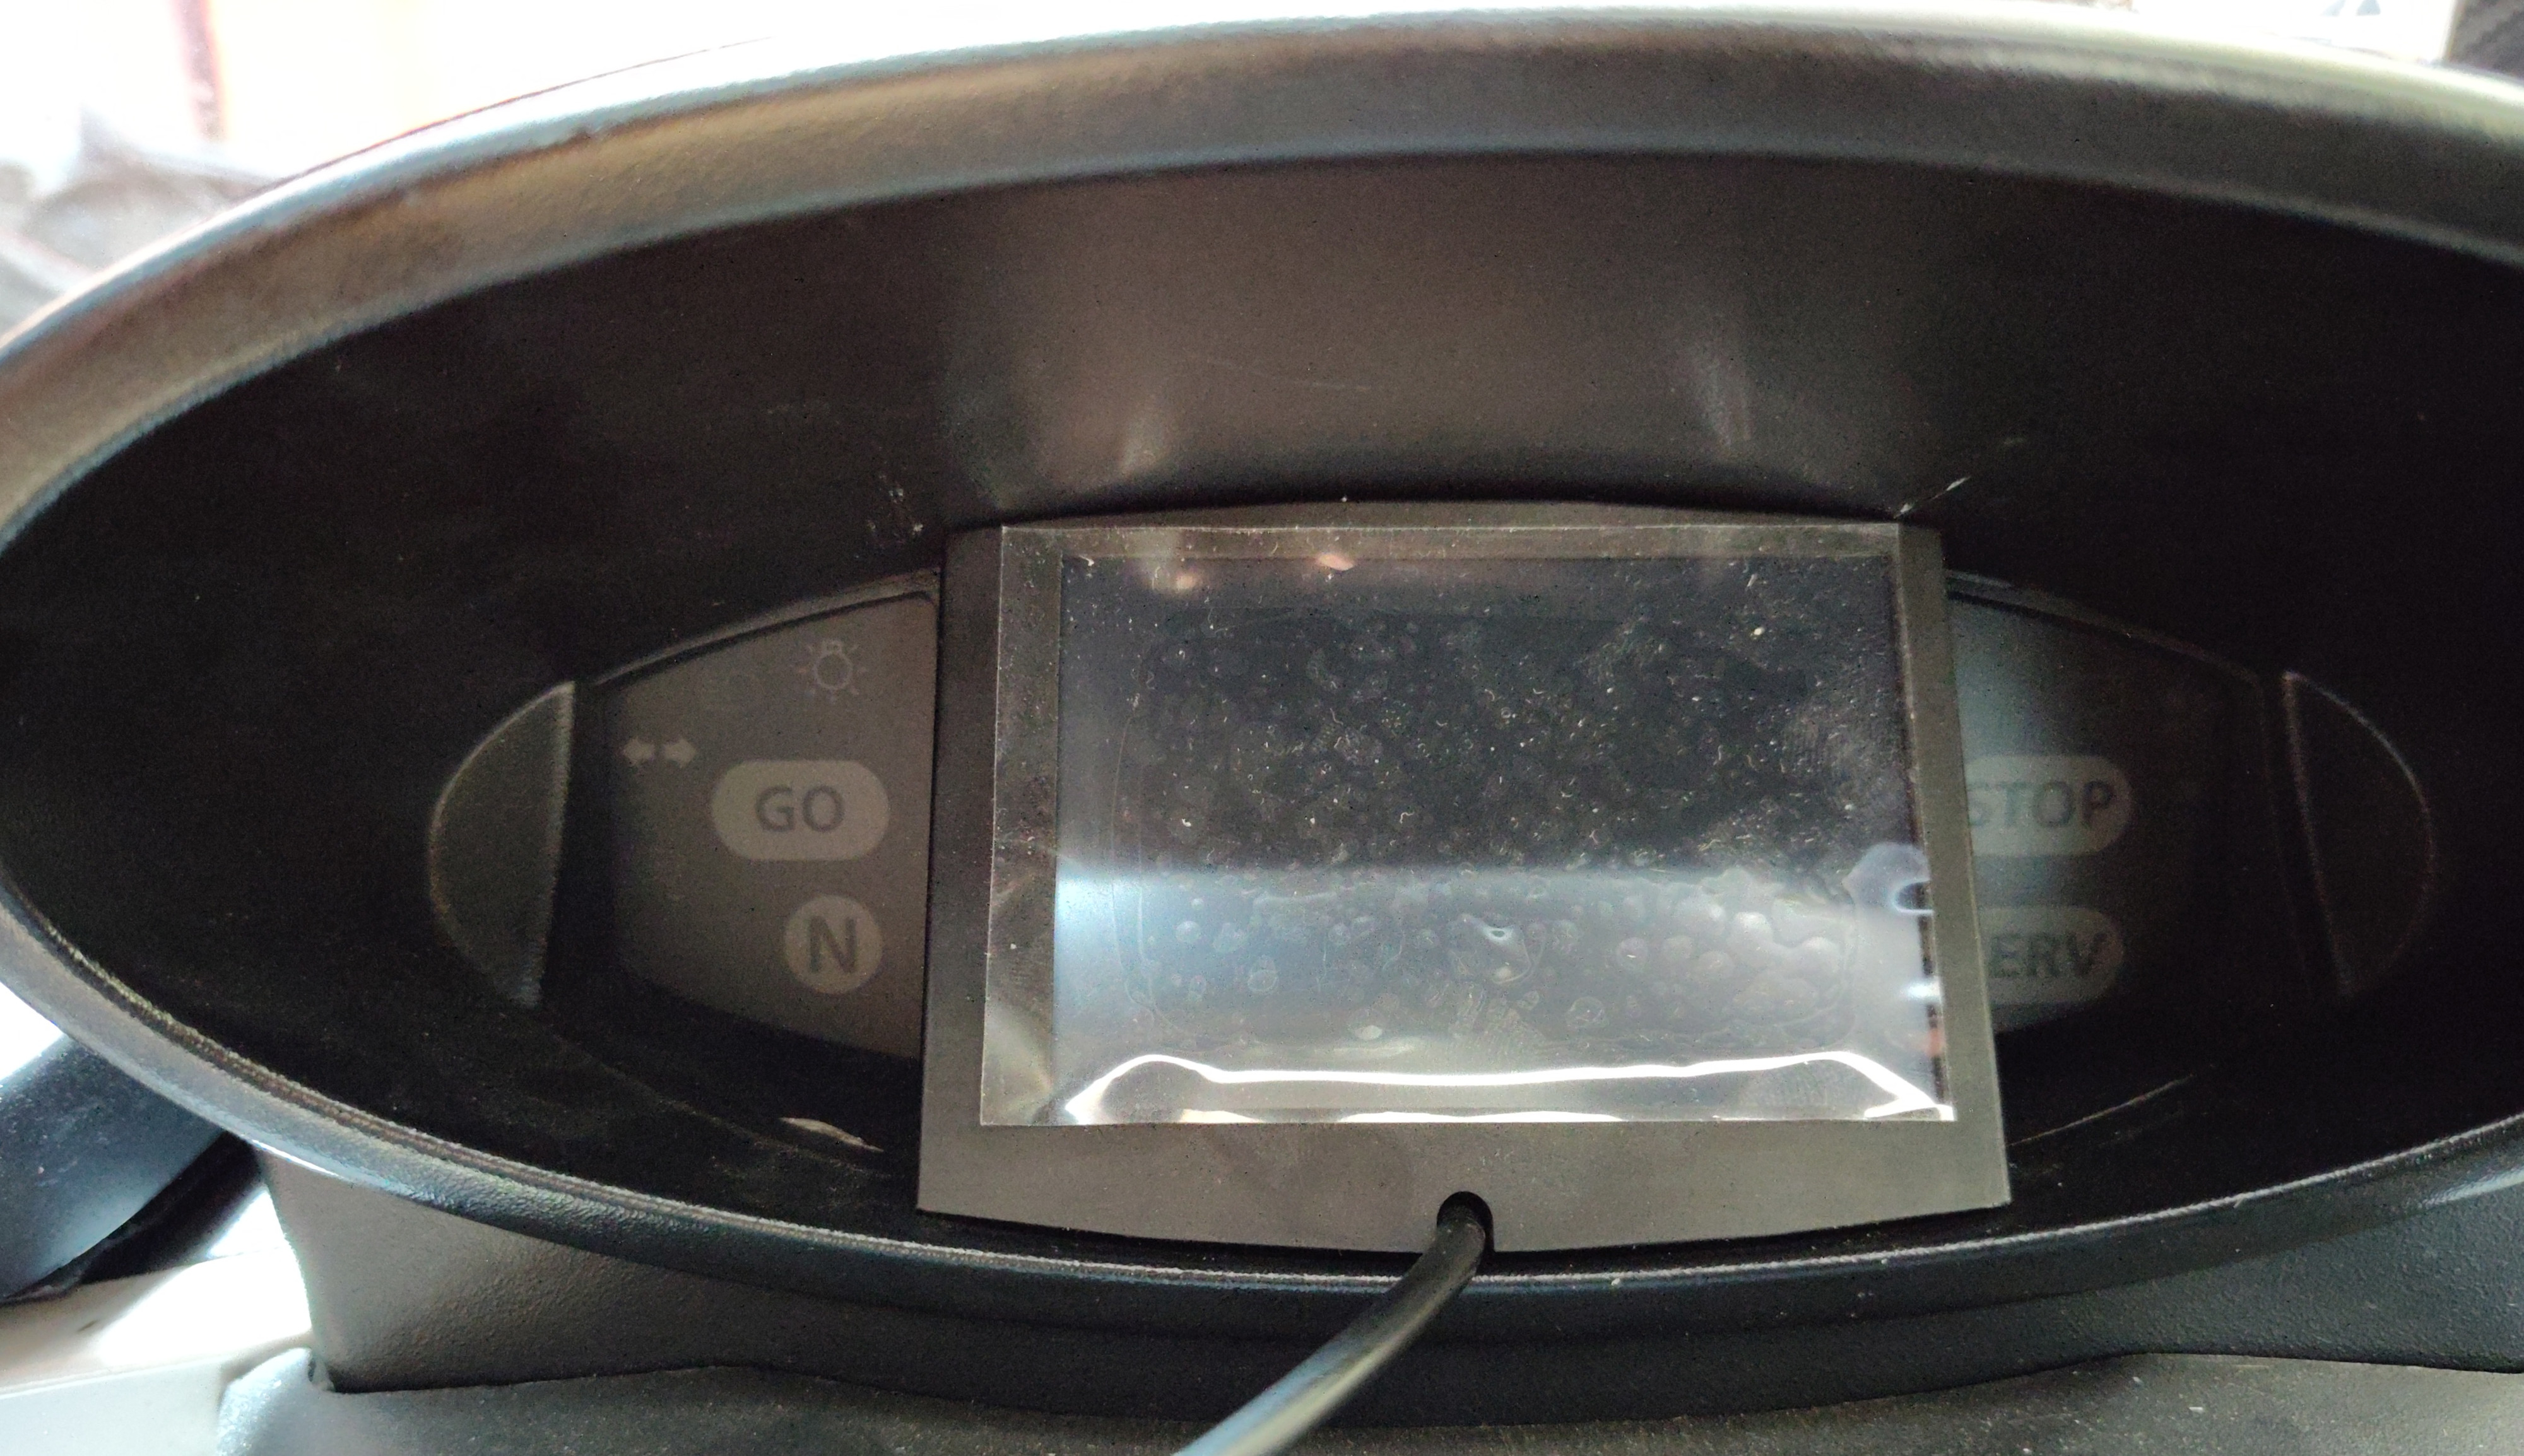
\includegraphics[width=0.8\textwidth]{figures/clip_on.jpg}
    \caption{Installation en mode à clipser}
\end{figure}

Assurez-vous que le câble n'est pas pincé dans la partie inférieure de l'écran et qu'il est libre de se déplacer dans l'orifice prévu à cet effet, sinon vous risqueriez d'endommager le câble.

\subsection{Mode support 3D}

S'il est fourni, vous pouvez utiliser le support 3D pour placer l'écran sur une surface plane à l'intérieur de la voiture.
Vous pouvez appliquer du ruban adhésif double face en dessous afin de le coller à la surface.
Ou vous pouvez utiliser les trous de vis sous le support pour le fixer à l'aide de deux vis.

Comme nous l'avons fait pour le mode à clipser, assurez-vous que le câble n'est pas pincé à l'arrière de l'écran lors de la mise en place du capot, mais qu'il est libre de se déplacer dans l'orifice prévu à cet effet, sinon vous risqueriez d'endommager le câble.
Reportez-vous à la Figure~\ref{fig:back_cover} et à la Figure~\ref{fig:bottom_cover_screwholes} à la page~\pageref{fig:back_cover} pour voir les pièces mentionnées.
Voici à quoi ressemble le support 3D sans l'écran installé.

\begin{figure}[H]
    \centering
    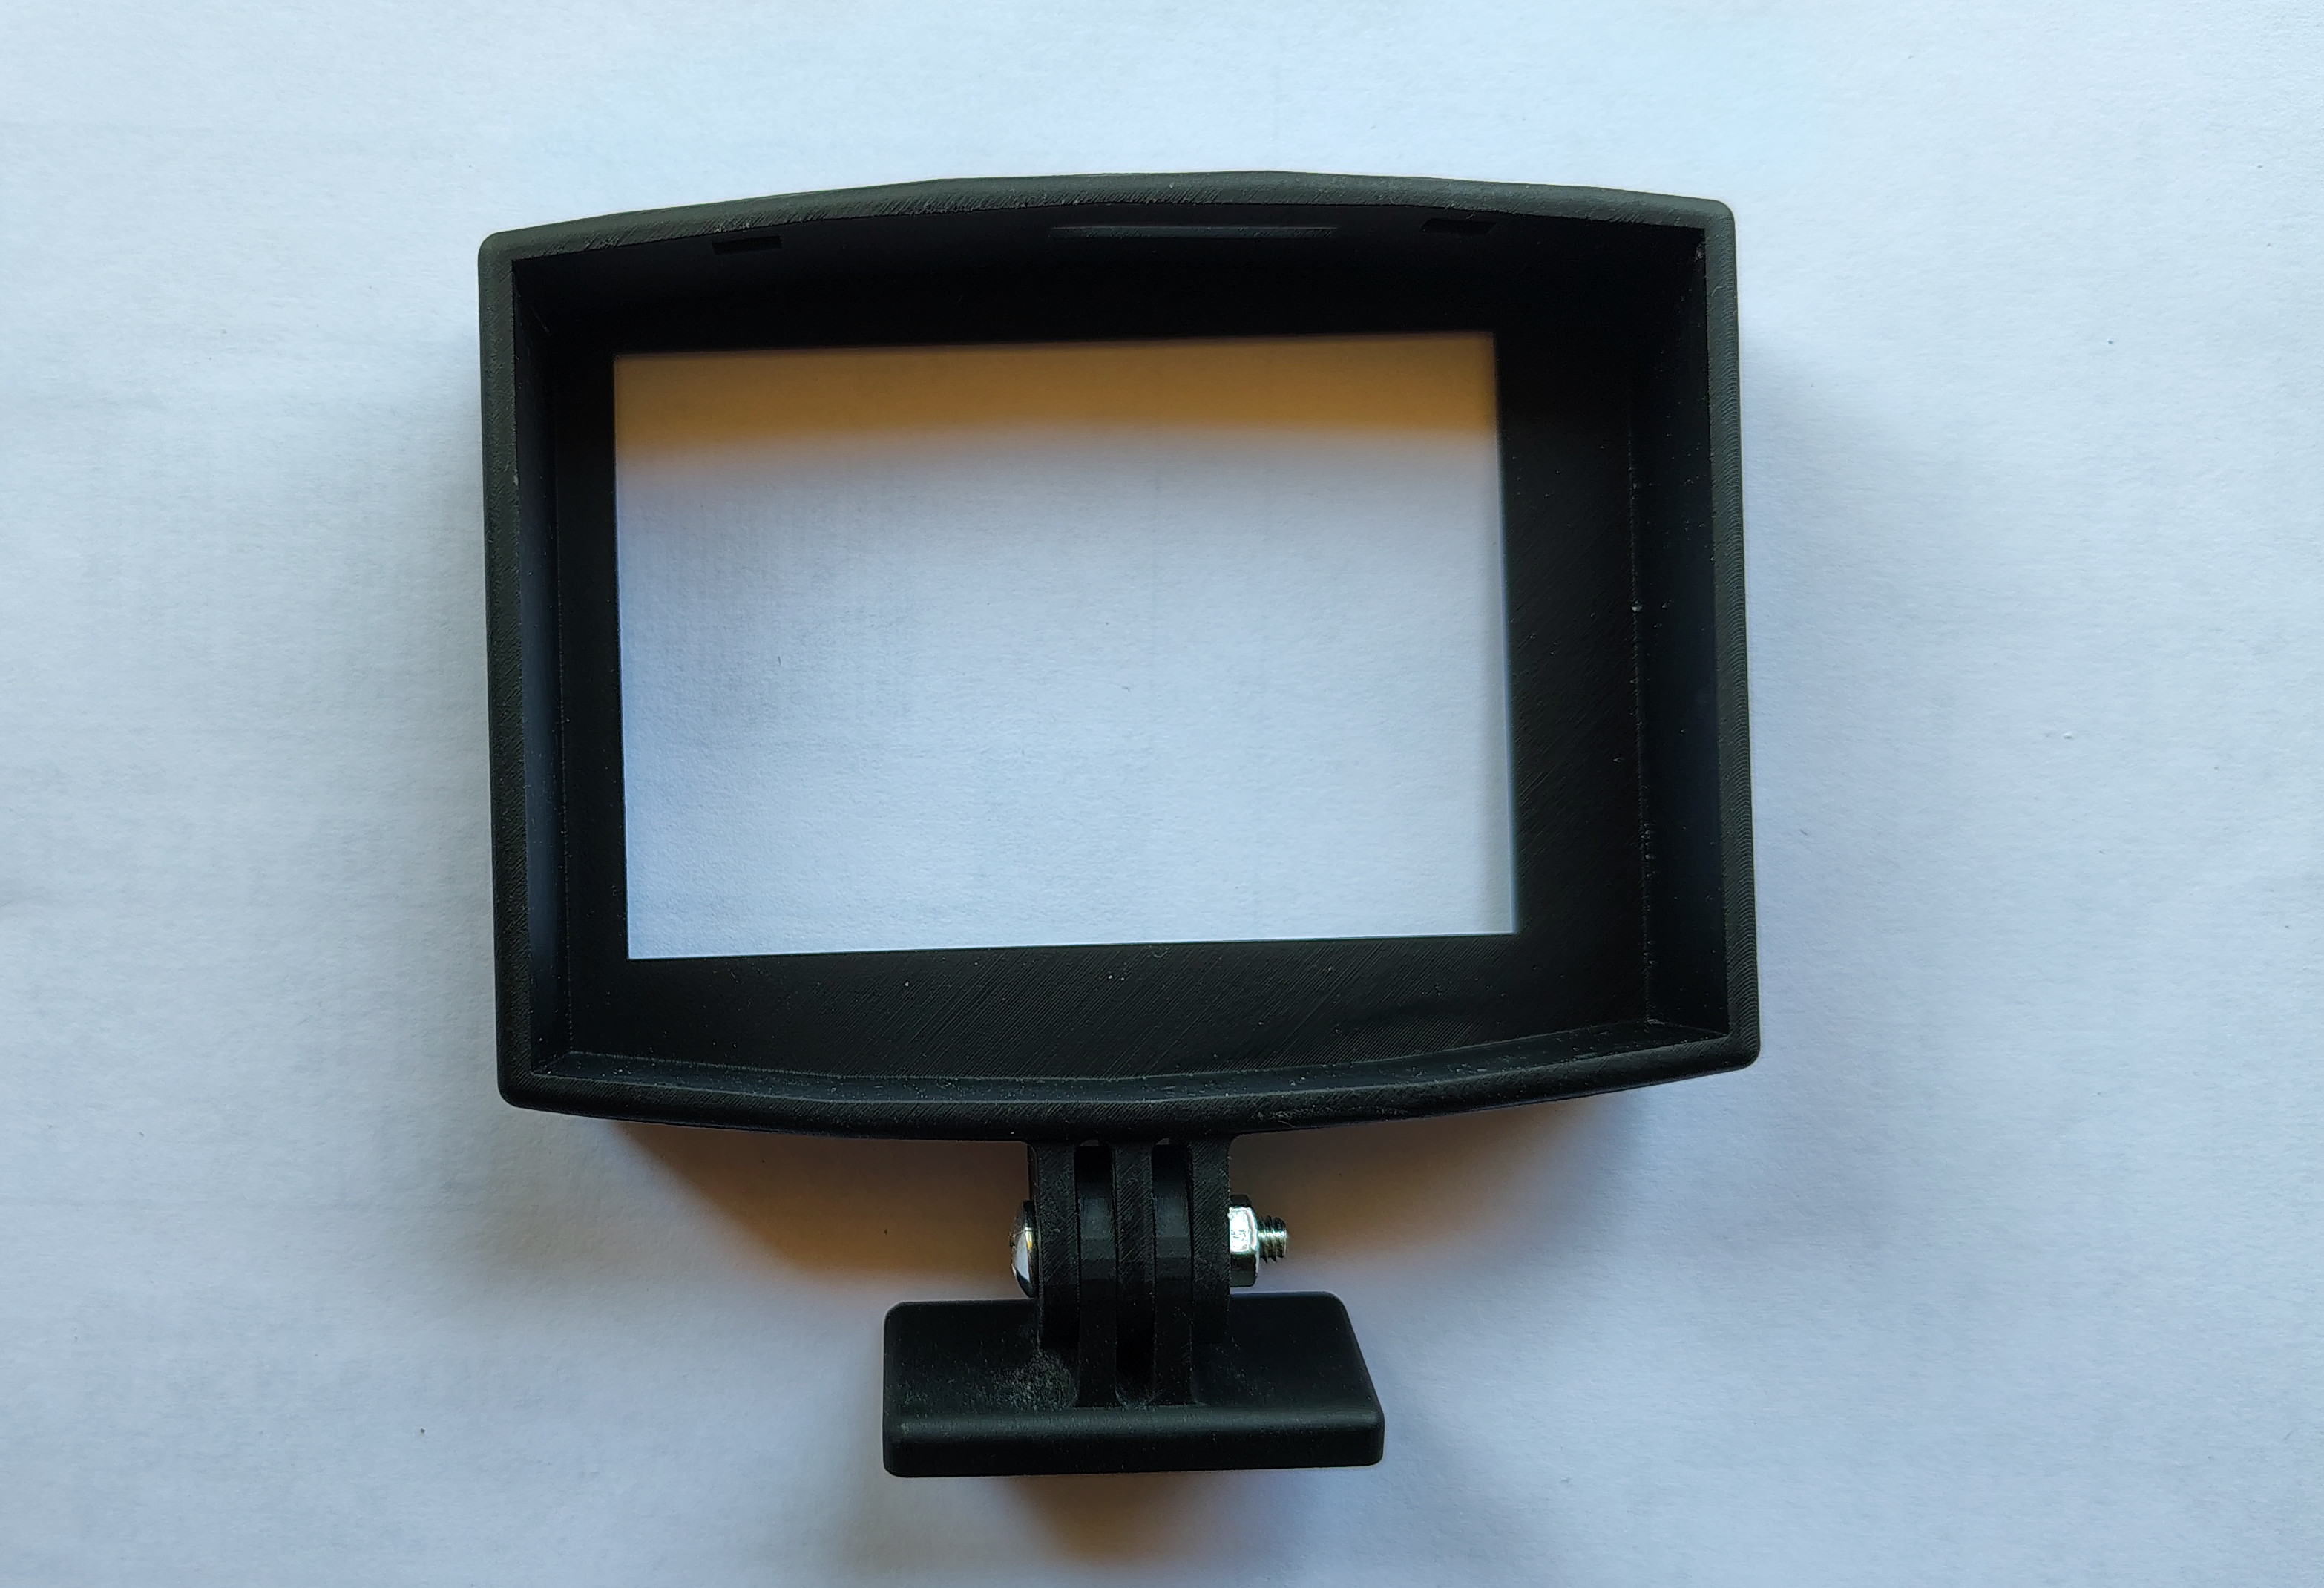
\includegraphics[width=0.8\textwidth]{figures/3d_stand.jpg}
    \caption{Support vide imprimé en 3D}
\end{figure}

\subsection{Raccordement du câble}

Vous pouvez ensuite retirer le film protecteur de l'écran et brancher le câble pour l'alimenter.
L'autre extrémité du câble doit être connectée au boîtier noir, qui sera installé lors de la prochaine étape.
Il ne s'insère que dans un seul sens, veillez donc à bien aligner le connecteur avant de le brancher.

\begin{figure}[H]
    \centering
    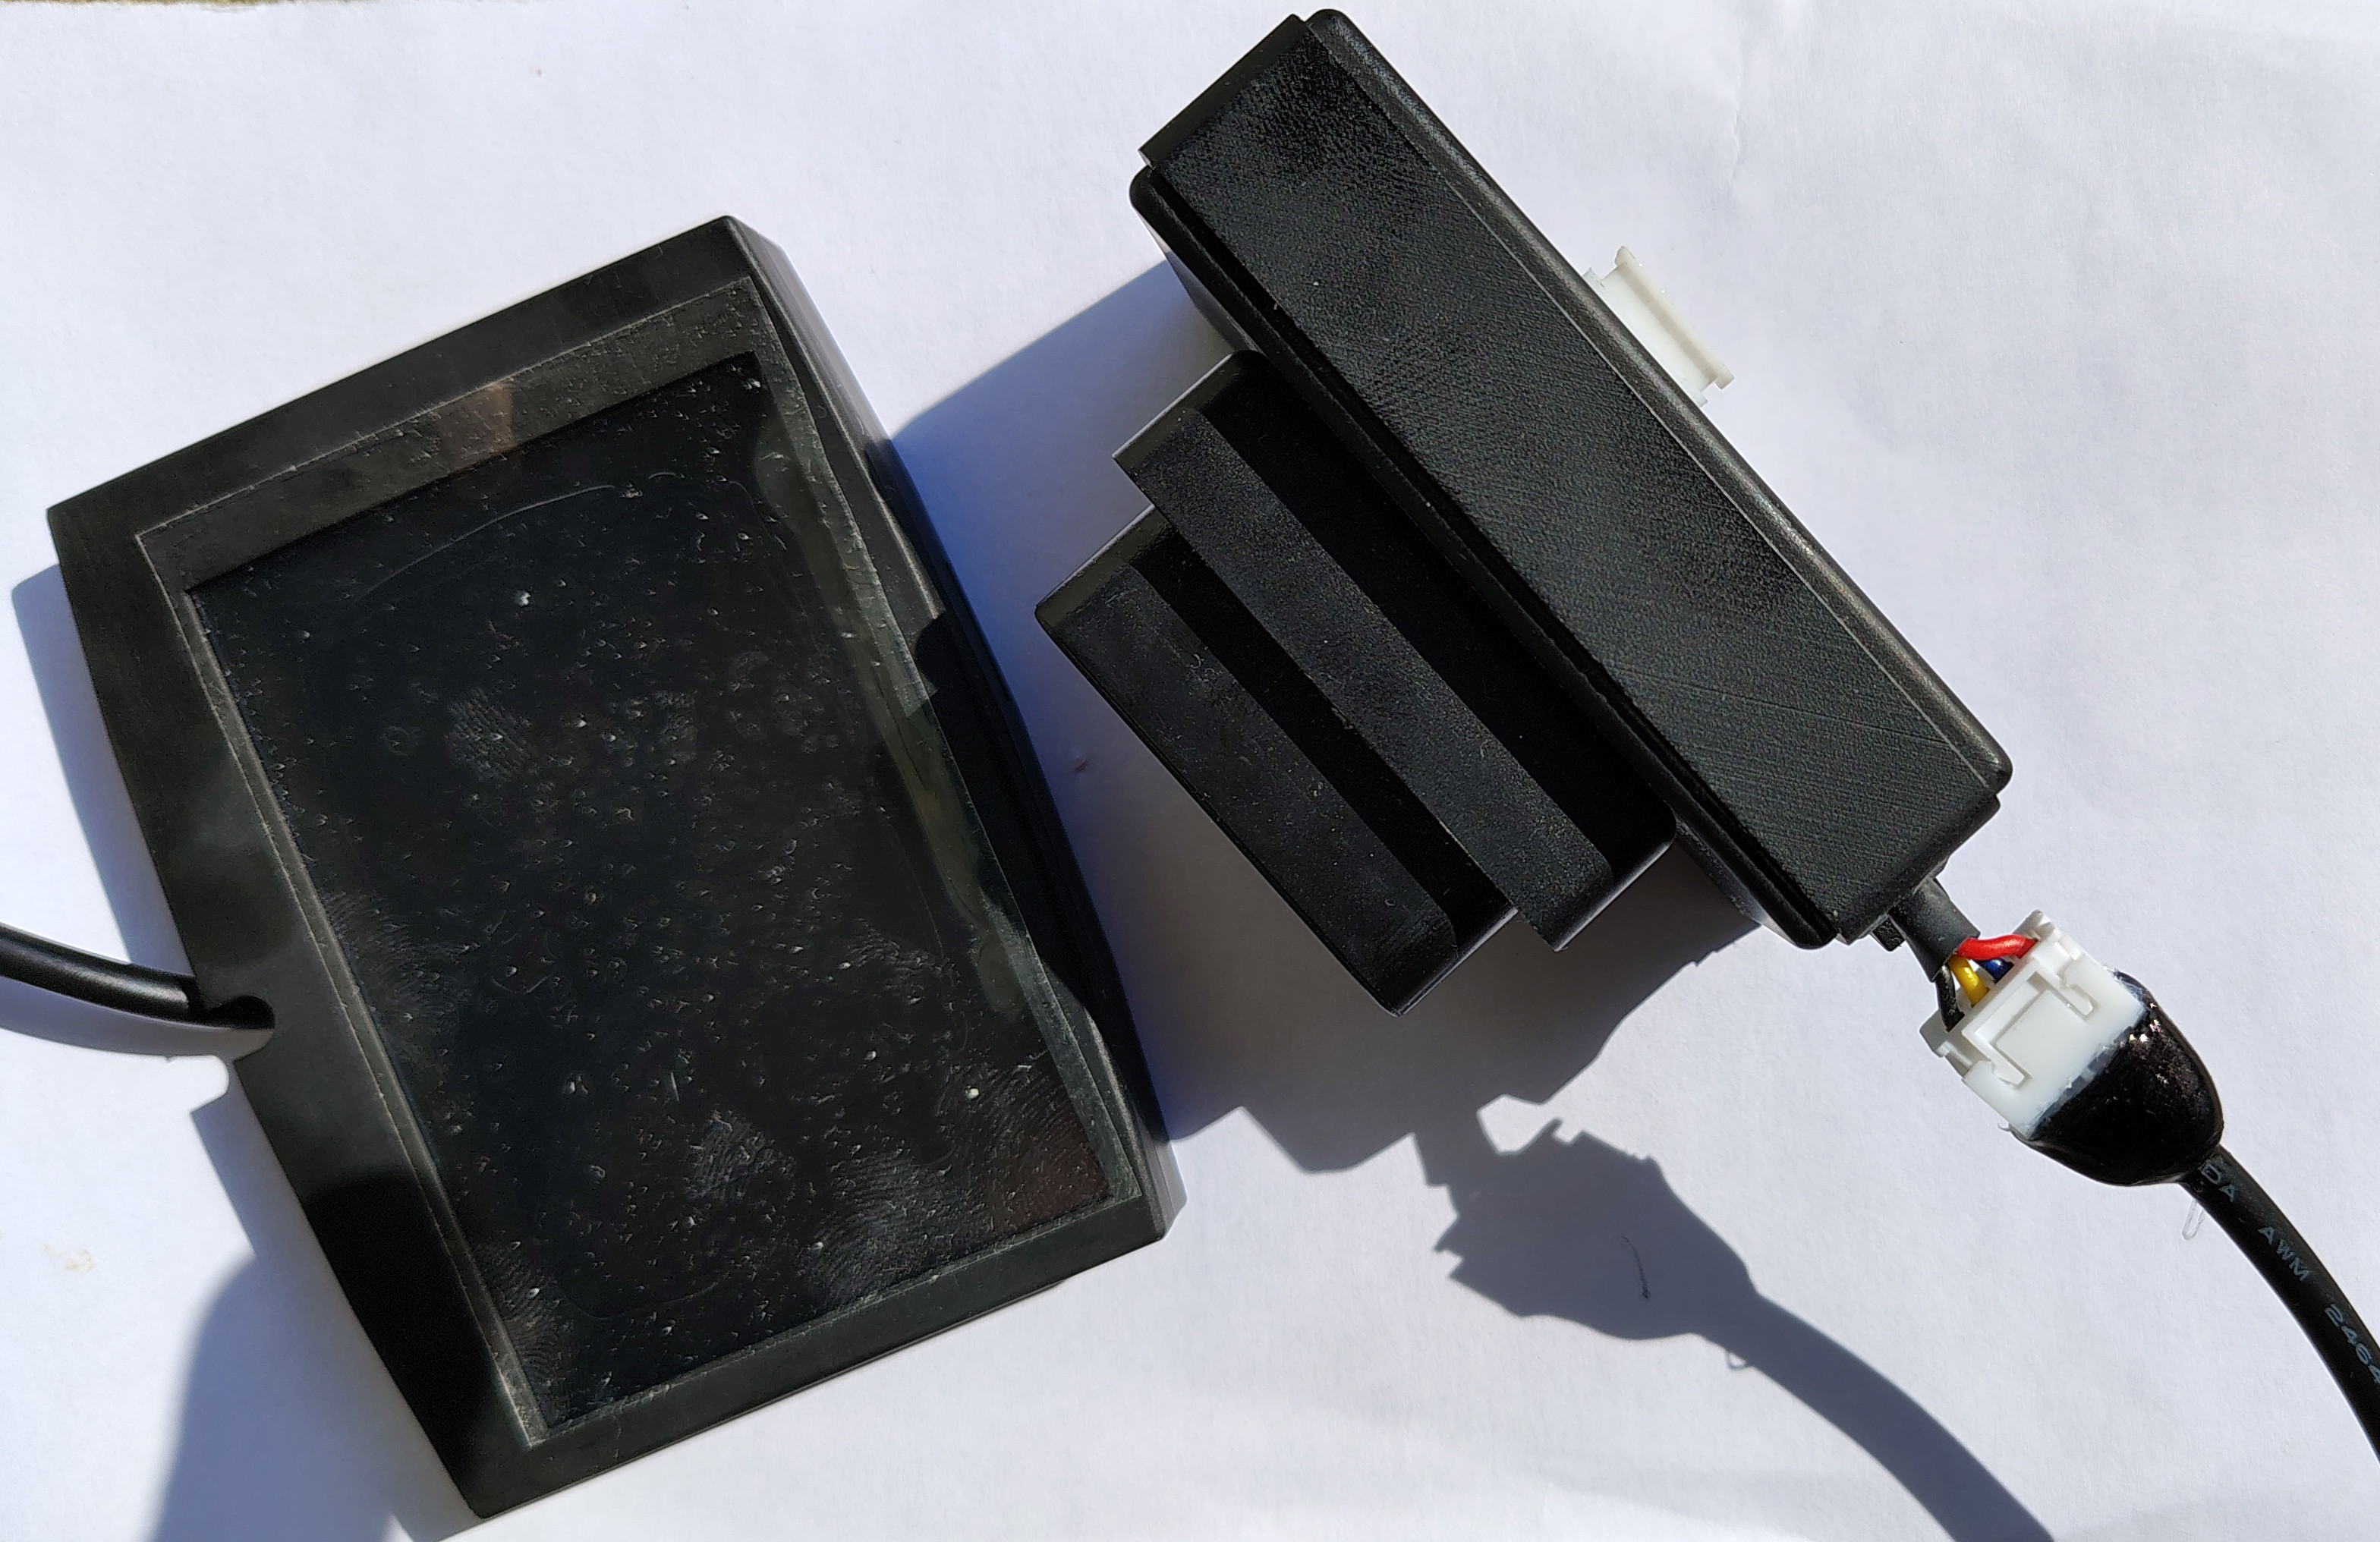
\includegraphics[width=0.8\textwidth]{figures/bb_connection.jpg}
    \caption{Connexion du boîtier noir}
\end{figure}

\section{Positionnement du boîtier noir}

Après avoir décidé où placer l'écran, vous devez brancher le boîtier noir.

Le boîtier noir doit être connecté à la prise OBD2 de la voiture, qui se trouve à l'intérieur de la boîte à gants gauche de la Twizy. Si vous ne l'avez jamais ouverte auparavant, vous trouverez un petit cache en plastique à retirer pour accéder au port OBD2. Une fois l'accès dégagé, branchez simplement le boîtier noir et assurez-vous qu'il est solidement connecté. Il ne s'insère que dans un seul sens, veillez donc à bien aligner le connecteur avant de le brancher.

\begin{figure}[H]
    \centering
    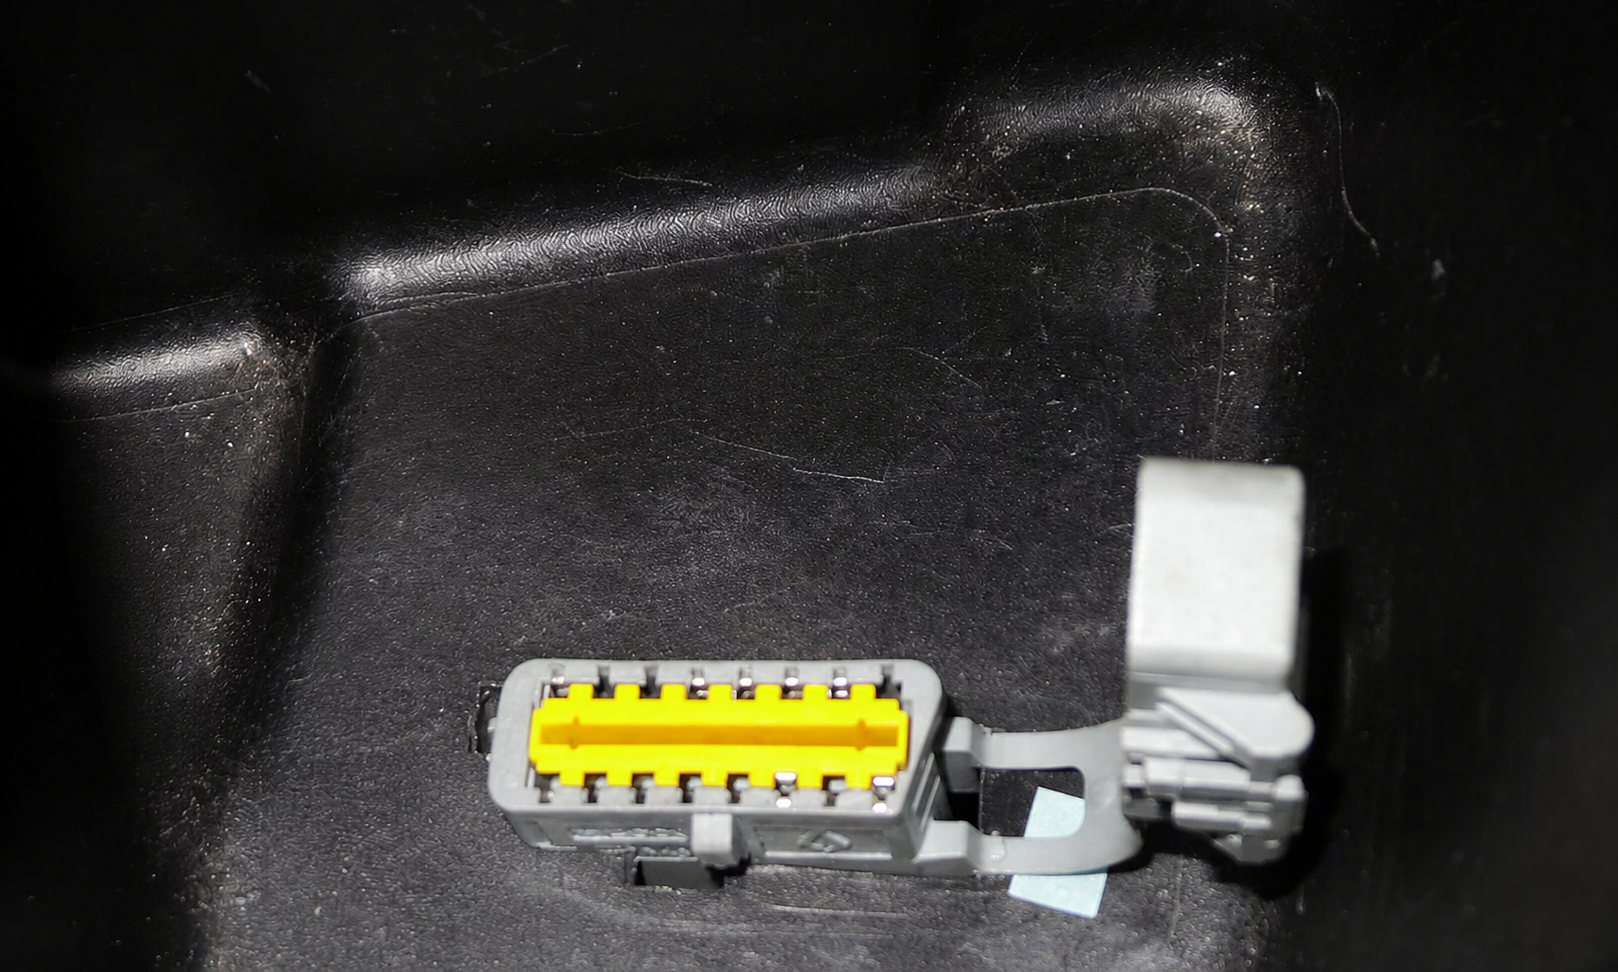
\includegraphics[width=0.8\textwidth]{figures/obd_connector.png}
    \caption{Emplacement du connecteur OBD2 dans la Twizy}
\end{figure}

\textbf{Ce n'est qu'après avoir connecté l'écran} que vous pourrez activer l'interrupteur du boîtier noir.
Et l'installation est terminée ! Vous pouvez maintenant démarrer votre Twizy et profiter des fonctionnalités du ToM+.
